\documentclass[8pt,landscape]{article}
\usepackage{multicol}
\usepackage{calc}
\usepackage{ifthen}
\usepackage{minted}
\usemintedstyle{vs}
\usepackage{enumitem}
\newcommand{\saskeyword}[1]{\textcolor{blue}{#1}}
\newenvironment{sasminted}{\VerbatimEnvi	ronment\begin{minted}[escapeinside=||,fontsize=\small,baselinestretch=1, samepage=true]{sas}}
 {\end{minted}}
 \usepackage{amsmath}
\usepackage{verbatim}
\usepackage[landscape]{geometry}
\usepackage{hyperref}
\usepackage{graphicx}

% To make this come out properly in landscape mode, do one of the following
% 1.
%  pdflatex latexsheet.tex
%
% 2.
%  latex latexsheet.tex
%  dvips -P pdf  -t landscape latexsheet.dvi
%  ps2pdf latexsheet.ps


% This sets page margins to .5 inch if using letter paper, and to 1cm
% if using A4 paper. (This probably isn't strictly necessary.)
% If using another size paper, use default 1cm margins.
\ifthenelse{\lengthtest { \paperwidth = 11in}}
	{ \geometry{top=.1in,left=.1in,right=.1in,bottom=.1in} }
	{\ifthenelse{ \lengthtest{ \paperwidth = 297mm}}
		{\geometry{top=1cm,left=1cm,right=1cm,bottom=1cm} }
		{\geometry{top=1cm,left=1cm,right=1cm,bottom=1cm} }
	}

% Turn off header and footer
\pagestyle{empty}
 

% Redefine section commands to use less space
\makeatletter
\renewcommand{\section}{\@startsection{section}{1}{0mm}%
                                {-1ex plus -.5ex minus -.2ex}%
                                {0.5ex plus .2ex}%x
                                {\normalfont\large\bfseries}}
\renewcommand{\subsection}{\@startsection{subsection}{2}{0mm}%
                                {-1explus -.5ex minus -.2ex}%
                                {0.5ex plus .2ex}%
                                {\normalfont\normalsize\bfseries}}
\renewcommand{\subsubsection}{\@startsection{subsubsection}{3}{0mm}%
                                {-1ex plus -.5ex minus -.2ex}%
                                {1ex plus .2ex}%
                                {\normalfont\small\bfseries}}
\renewcommand{\baselinestretch}{0.7} 
\makeatother

% Define BibTeX command
\def\BibTeX{{\rm B\kern-.05em{\sc i\kern-.025em b}\kern-.08em
    T\kern-.1667em\lower.7ex\hbox{E}\kern-.125emX}}

% Don't print section numbers
\setcounter{secnumdepth}{0}


\setlength{\parindent}{0pt}
\setlength{\parskip}{0pt}
\setitemize{noitemsep,topsep=0pt,parsep=0pt,partopsep=0pt}


% -----------------------------------------------------------------------

\begin{document}

\raggedright
\footnotesize
\begin{multicols}{3}


% multicol parameters
% These lengths are set only within the two main columns
%\setlength{\columnseprule}{0.25pt}
\setlength{\premulticols}{1pt}
\setlength{\postmulticols}{1pt}
\setlength{\multicolsep}{1pt}
\setlength{\columnsep}{2pt}

\begin{center}
     \Large{\textbf{CS3210 Cheat Sheet}} \\
\end{center}

\section{Chapter 2}
\subsection{Primatives}
\begin{itemize}
	\item Locks
	\item Semaphores - Binary/Mutex and Counting (Wait, Signal)
	\item Condition Variables (Wait, Signal, Broadcast)
	\item Monitors (Mutex + CV)
	\item Barrier
	\item Starvation, Deadlock
\end{itemize}

\subsection{Producer-consumer with finite buffer}
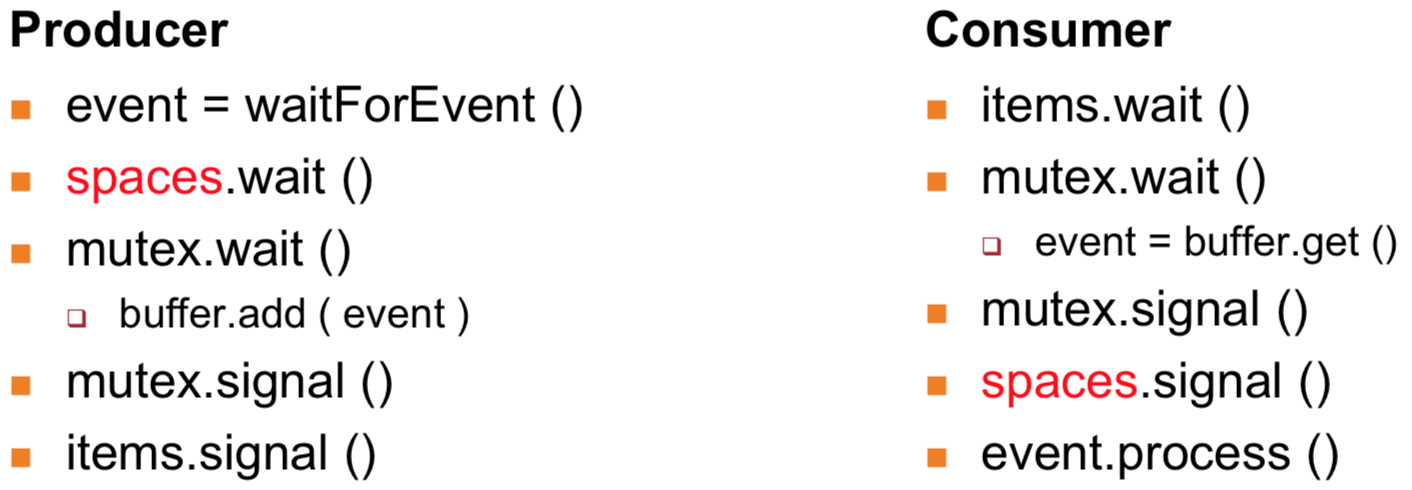
\includegraphics[scale=0.3]{./prod-cons}

\subsection{Lightswitch Definition}
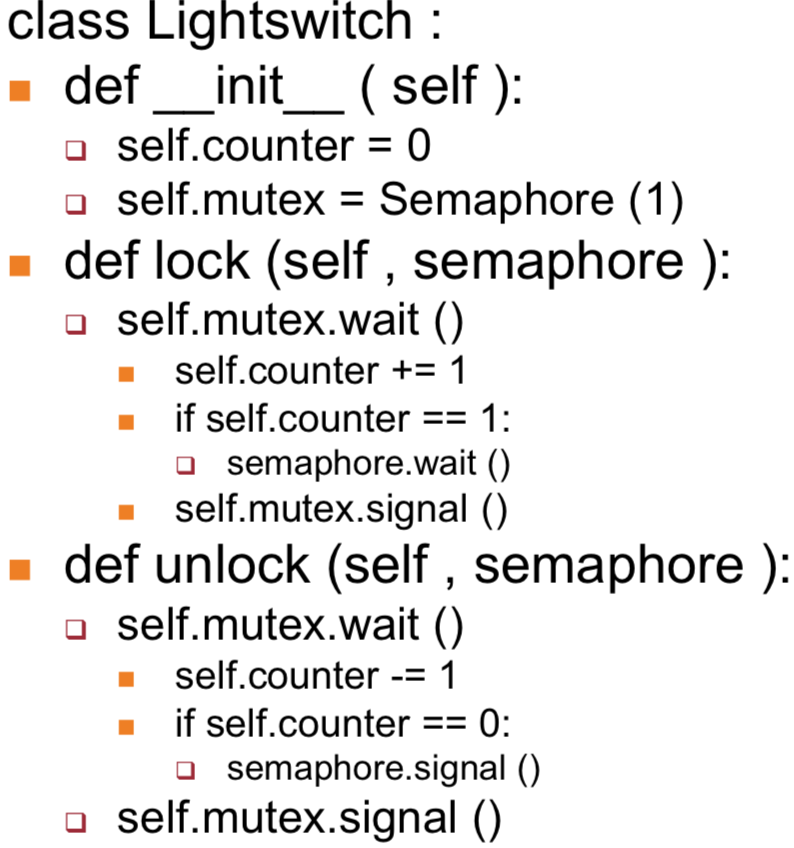
\includegraphics[scale=0.3]{./lightswitch}

\subsection{Readers-Writers Turnstile}
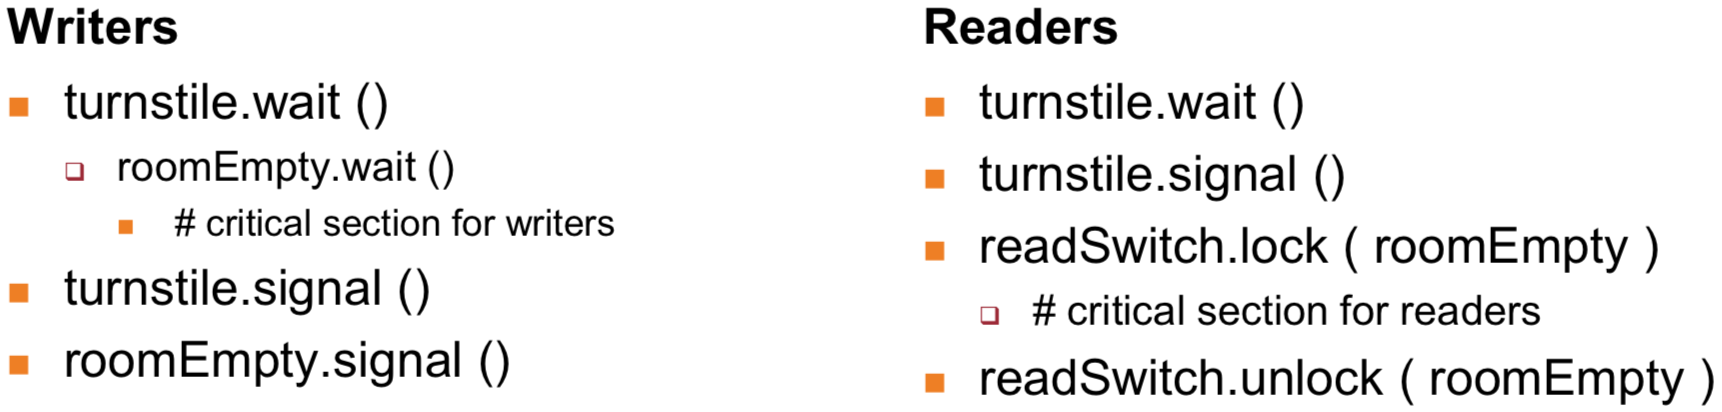
\includegraphics[scale=0.3]{./rwts}

\subsection{Readers-Writers with priorities}
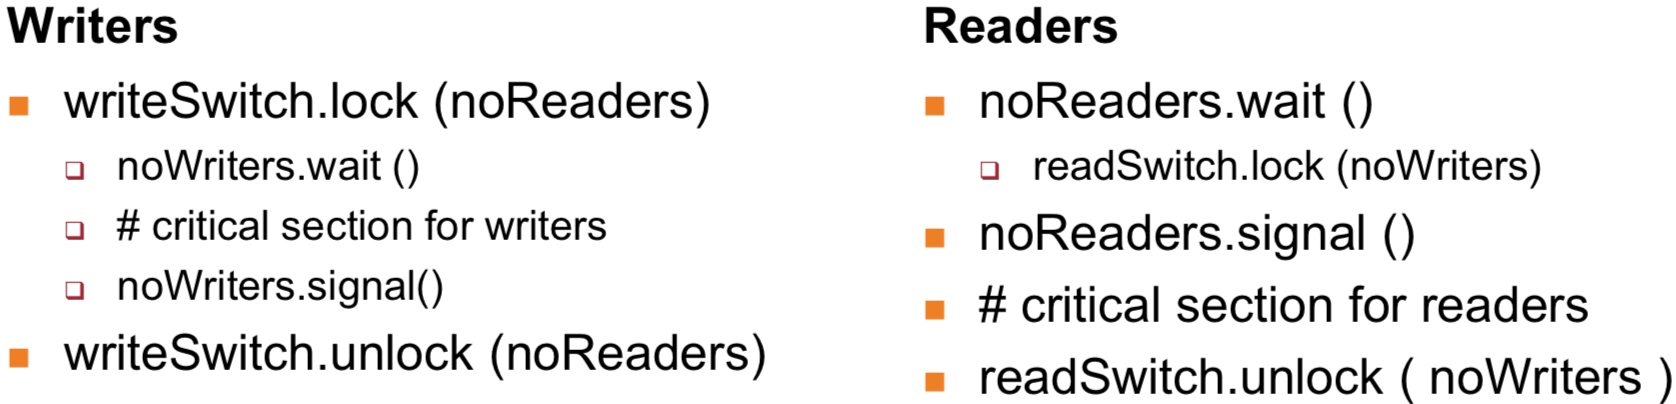
\includegraphics[scale=0.3]{./rwprior}

\section{Chapter 3}
\subsection{Levels of Parallelism}
\begin{itemize}
	\item Single Processor:
		 \begin{itemize}[label=$\circ$]
		 	\item Bit Level
			\item Instruction Level
			\item Thread Level
			\item Process Level
		\end{itemize}
	\item Multiple Processors:
		\begin{itemize}[label=$\circ$]
			\item Prcessor Level
		\end{itemize}
\end{itemize}

\subsection{Bit Level}
Word size (16-bit, 32-bit, 64-bit)

\subsection{Instruction Level}
\begin{enumerate}
	\item Pipelining - split instruction execution into multiple stages, then allow multiple instructions to occupy different stages in the same clock cycle; number of pipeline stages == maximum achievable speedup
	\item Superscalar - duplicate pipelines, allow multiple instructions to pass through the same stage
\end{enumerate}

\subsection{Thread Level Parallelism}
\begin{itemize}
	\item Simultaneous Multi-threading - Hyper-threading; Run multiple (2) threads at the same time
\end{itemize}

\subsection{Process Level Parallelism}
\begin{itemize}
	\item Instead of multiple threads, can use multiple processes to work in parallel.
	\item Each process needs an independent set of processor context $\rightarrow$ can be mapped to multiple processor cores
\end{itemize}

\subsection{Flynn's Taxonomy}
\begin{itemize}
	\item Single Instruction Single Data (SISD)
	\item Single Instruction Multiple Data (SIMD) - SSE, AVX instructions
	\item Multiple Instruction Single Data (MISD) - Space Shuttle
	\item Multiple Instruction Multiple Data (MIMD) - multiprocessor
\end{itemize}

\subsection{Memory Organization}
\begin{itemize}
	\item Distributed-Memory Multicomputers: 		
		\begin{itemize}[label=$\ast$]
			\item Memory in a node is private, use message-passing to exchange data
		\end{itemize}
	\item Shared-memory Multiprocessors
		\begin{itemize}[label=$\ast$]
			\item Data-exchanges between nodes through shared variables
		\end{itemize}
		\begin{itemize}[label=$\circ$]
			\item Uniform Memory Access (UMA)
				\begin{itemize}[label=$\ast$]
					\item Latency of accessing main memory is same for all processors
					\item Main memory is congregated at some other area separate from processors
				\end{itemize}
			\item Non-Uniform Memory Access (NUMA)		
				\begin{itemize}[label=$\ast$]
					\item Also known as distributed SHARED-MEMORY
					\item Physically distributed memory of all processing elements combined to form a global shared-memory address space
					\item Access local memory is fater than remote memory for a processor $\rightarrow$ non-uniform access time
					\item Related: Cache Coherent NUMA (ccNUMA) - Each node has cache memory to reduce contention
				\end{itemize}
			\item Cache-only Memory Access (COMA)
				\begin{itemize}[label=$\ast$]
					\item Quite similar to NUMA, replace memory with a cache
					\item Data migrates dynamically and continuously according to cache coherence scheme
				\end{itemize}
		\end{itemize}
	\item Hybrid (Distributed-Shared Memory)
\end{itemize}

\subsection{Shared Memory Systems}
\begin{itemize}
	\item Advantages
		\begin{itemize}[label=$\circ$]
			\item No need to partition code or data
			\item No need to physically move data among processors $\rightarrow$ communication is efficient
		\end{itemize}
	\item Disadvantages
		\begin{itemize}[label=$\circ$]
			\item Special synchronization constructions required
			\item Lack of scalability due to contention
		\end{itemize}
\end{itemize}

\subsection{Multicore Architecture}
\begin{itemize}
	\item Hierachical design
	\item Pipelined design
	\item Network-based design - Interconnection networks
\end{itemize}

\section{Chapter 4}
What limits parallelism? Dependencies, Overheads in parallelism (context switching), Synchronization

\subsection{Instruction Parallelism}
\begin{itemize}
	\item Flow dependency - Read after Write, aka True dependency
	\item Anti-dependency - Write after Read
	\item Output dependency - Write after Write
\end{itemize}

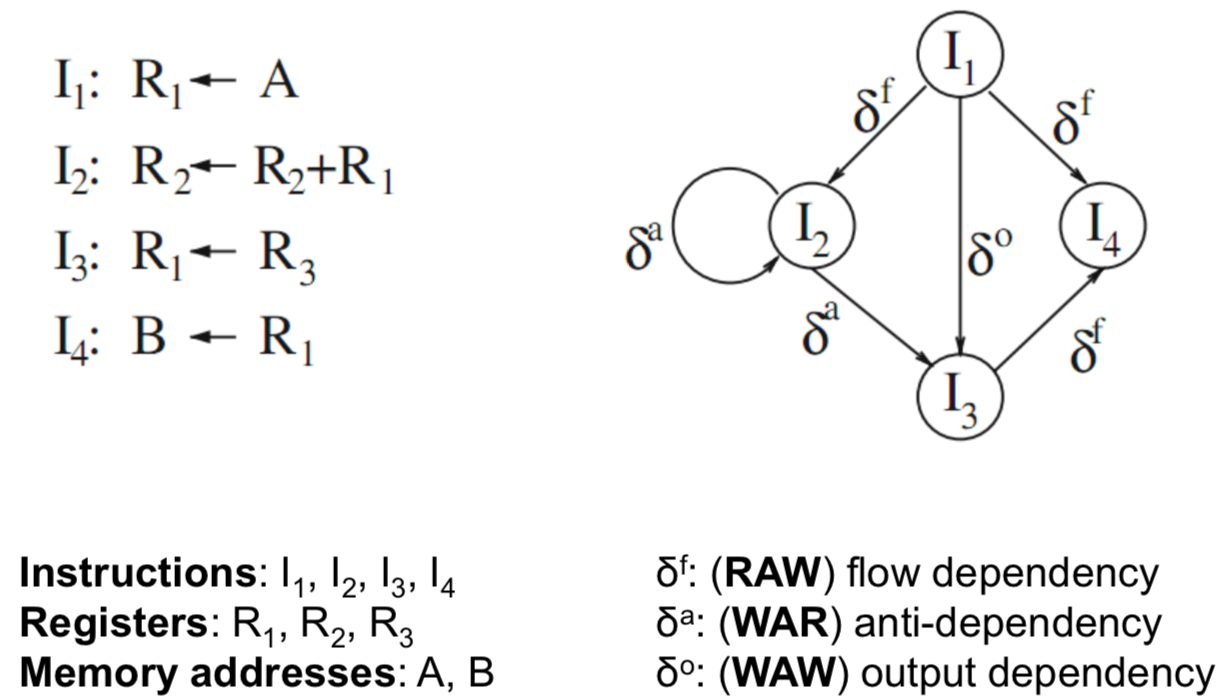
\includegraphics[scale=0.38]{./data_dep_graph}

\subsection{Loop Parallelism}

\subsection{Data Parallelism}
\begin{itemize}
	\item Partition the data used in solving the problem among the processing units; each processing unit carries out similar operaitons on its part of the data.
	\item SIMD computers / instructions exploit data parallelism
	\item (Data Parallelism on MIMD) SPMD (Single Program Multiple Data) - one parallel program executed by all processors in parallel (both shared and distributed address space); example is MPI
\end{itemize}

\subsection{Task Parallelism}
\begin{itemize}
	\item Partition the tasks in solving the problem among the processing units
	\item Example: Different components of an SQL statement
\end{itemize}

\subsection{Task Dependence Graph}
\begin{itemize}
	\item Critical Path Length: Minimum (slowest) completion time
	\item Degree of concurrency = Total Work / Critical Path Length
\end{itemize}

\subsection{Parallel Programming Patterns}
\begin{itemize}
	\item Fork-Join
	\item Parbegin-Parend - OpenMP
	\item SIMD - SSE instruction treats xmm registers (128 bit) as 4 32-bit floating point values
	\item SPMD - MPI
	\item Master-slave
	\item Client-Server (MPMD model)
	\item Pipelining
	\item Task (Work) Pools
	\item Producer-Consumer
\end{itemize}

\section{Chapter 5}
\subsection{CPU Time (No memory miss)}
\begin{equation}
\textrm{Time}_{\textrm{user}}(A) = N_{\textrm{cycle}}(A) \times \textrm{Time}_{\textrm{cycle}}
\end{equation}
\begin{equation}
N_{\textrm{cycle}}(A) = \sum_{i=1}^{n} n_{i}(A) \times \textrm{CPI}_{i}
\end{equation}
\begin{equation}
\textrm{Time}_{\textrm{user}}(A) = N_{\textrm{instructions}}(A) \times \textrm{CPI}(A) \times \textrm{Time}_{\textrm{cycle}}
\end{equation}

\subsection{CPU Time (With memory miss)}
\subsubsection{Memory Access Time}
\begin{equation}
\textrm{Time}_{\textrm{user}}(A) = \left( N_{\textrm{cycle}}(A) + N_{\textrm{mm\_cycle}}(A)  \right) \times \textrm{Time}_{\textrm{cycle}}
\end{equation}
\textbf{Consider a one-level cache:}
\begin{equation}
N_{\textrm{mm\_cycle}}(A) = N_{\textrm{read\_cycle}}(A) + N_{\textrm{write\_cycle}}(A)
\end{equation}
\begin{equation}
N_{\textrm{read\_cycle}}(A) = N_{\textrm{read\_op}}(A) \times R_{\textrm{read\_miss}}(A) \times N_{\textrm{miss\_cycles}}(A)
\end{equation}
\begin{equation}
N_{\textrm{write\_cycle}}(A) = N_{\textrm{write\_op}}(A) \times R_{\textrm{write\_miss}}(A) \times N_{\textrm{miss\_cycles}}(A)
\end{equation}

\subsubsection{Refinement with Memory Access Time}
\begin{equation}
\resizebox{.33 \textwidth}{!} 
{
    $ \textrm{Time}_{\textrm{user}}(A) = \left( N_{\textrm{instructions}}(A) \times \textrm{CPI}(A)
+ N_{\textrm{rw\_op}}(A) \times R_{\textrm{rw\_miss}}(A) \times N_{\textrm{rw\_cycles}}(A) \right) \times \textrm{Time}_{\textrm{cycle}} $
}
\end{equation}


\subsubsection{Average Memory Access Time}
Average read access time = Time for read hit + Time for read miss
\begin{equation}
T_{\textrm{read\_access}}(A) = T_{\textrm{read\_hit}}(A) + R_{\textrm{read\_miss}}(A) \times T_{\textrm{read\_miss}}(A)
\end{equation}
Two-level Cache example:
\begin{equation}
T_{\textrm{read\_access}}(A) = T_{\textrm{read\_hit}}^{L1}(A) + R_{\textrm{read\_miss}}^{L1}(A) \times T_{\textrm{read\_miss}}^{L1}(A)
\end{equation}
\begin{equation}
T_{\textrm{read\_miss}}^{L1}(A) = T_{\textrm{read\_hit}}^{L2}(A) + R_{\textrm{read\_miss}}^{L2}(A) \times T_{\textrm{read\_miss}}^{L2}(A)
\end{equation}
Global Miss Rate:
\begin{equation}
R_{\textrm{read\_miss}}^{L1}(A) \times R_{\textrm{read\_miss}}^{L2}(A)
\end{equation}

\subsection{MIPS, MFLOPS}
\begin{equation}
MIPS(A) = \frac{N_{\textrm{instr}}(A)}{\textrm{Time}_{\textrm{user}}(A) \times 10^{6}} = \frac{\textrm{clock\_frequency}}{CPI(A) \times 10^{6}}
\end{equation}
\begin{equation}
MFLOPS(A) = \frac{N_{\textrm{fl\_ops}}(A)}{\textrm{Time}_{\textrm{user}}(A) \times 10^{6}}
\end{equation}

\subsection{Parallel Execution Time}
\begin{itemize}
	\item $T_{p}(n)$ - time for $p$ processors to work on problem of size $n$
\end{itemize}
\begin{equation}
C_{p}(n) = p \times T_{p}(n)
\end{equation}
\begin{itemize}
	\item $C_{p}(n)$ - cost of a parallel program with input size $n$ executed on $p$ processors
	\item Parallel program is cost optimal if it executes the same total number of operations as the fastest sequential program
\end{itemize}
\begin{equation}
S_{p}(n) = \frac{T_{best\_seq}(n)}{T_{p}(n)}
\end{equation}
\begin{itemize}
	\item $S_{p}(n)$ is the speedup of the parallel program on $p$ processors
	\item Theoretically $S_{p}(n) \leq p$ always holds
	\item In practice $S_{p}(n) > p$ can occur due to better cache locality, early termination
\end{itemize}
\begin{equation}
E_{p}(n) = \frac{T_{*}(n)}{C_{p}(n)} = \frac{S_{p}(n)}{p} = \frac{T_{*}(n)}{p \times T_{p}(n)}
\end{equation}
\begin{itemize}
	\item Use $T_{*}(n)$ as a shorthand for $T_{best\_seq}(n)$
	\item Efficiency measures the actual degree of speedup performance achived compared to the maximum
	\item In an ideal speedup $S_{p}(n) = p \rightarrow E_{p}(n) = 1$
\end{itemize}

\subsection{Parallel Laws}
\subsubsection{Amdahl's Law}
\begin{itemize}
	\item Speedup of parallel execution is limited by the fraction of the algorithm that cannot be parallelized, $f$
	\item $f (0 \leq f \leq 1)$ - the sequential fraction
	\item "Fixed-workload" performance
\end{itemize}

\begin{equation}
S_{p}(n) = \frac{T_{*}(n)}{f \times T_{*}(n) + \frac{1-f}{p}T_{*}(n)} = \frac{1}{f + \frac{1-f}{p}} \leq \frac{1}{f}
\end{equation}
\begin{equation}
S_{p}(n) = \frac{p}{1 + (p-1) f}
\end{equation}

\subsubsection{Gustafson's Law}
\begin{itemize}
	\item In many computing problems, $f$ is not a constant
	\item Depends on problem size $n$: $f$ is a function of $n$, $f(n)$
	\item An effective parallel algorithm is: \begin{equation}
		\lim_{n\rightarrow\infty} f(n) = 0
	\end{equation}
	\item Thus speedup: \begin{equation}
		\lim_{n\rightarrow\infty} S_{p}(n) = \frac{p}{1 + (p-1)f(n)} = p
	\end{equation}
	\item In such cases, we can have \begin{equation}
		S_{p}(n) \leq p
	\end{equation}
\end{itemize}

\begin{equation}
S_{p}(n) = \frac{\tau_{f} + \tau_{v}(n, 1)}{\tau_{f} + \tau_{v}(n, p)}
\end{equation}

Assume parallel program is perfectly parallelizable (without overheads):
\begin{equation}
\tau_{v}(n, 1) = T^{*}(n) - \tau_{f} \  \textrm{and} \ \tau_{v}(n, p) = \frac{T^{*}(n) - \tau_{f}}{p}
\end{equation}
\begin{equation}
S_{p}(n) = \frac{\tau_{f} + T^{*}(n) - \tau_{f}}{\tau_{f} + \frac{T^{*}(n) - \tau_{f}}{p}} = \frac{\frac{\tau_{f}}{T*(n) - \tau_{f}} + 1}{\frac{\tau_{f}}{T^{*}(n) - \tau_{f}} + \frac{1}{p}}
\end{equation}
If $T*(n)$ increase strongly monotonically with $n$, then \begin{equation}
\lim_{n\rightarrow\infty} S_{p}(n) = p
\end{equation}

\section{Chapter 6}
\subsection{Memory Consistency Models}
\subsubsection{Relaxed Consistency}
\begin{itemize}
	\item Only if instructions operate on different memory locations
	\item Write-to-Read Program Order
	 	\begin{itemize}[label=$\circ$]
			\item Total Store Ordering (TSO)
			\item Processor Consitency (PC)
		\end{itemize}
	\item Write-to-Write Program Order
		\begin{itemize}[label=$\circ$]
			\item Partial Store Ordering (PSO)
		\end{itemize}
\end{itemize}

\subsubsection{TSO}
\begin{itemize}
	\item Can reorder W $\rightarrow$ R
	\item All processors see updates in the same order
\end{itemize}

\subsubsection{PC}
\begin{itemize}
	\item Can reorder W $\rightarrow$ R
	\item Different processors can see updates in different orders
	\item \textbf{Note:} Ordering should still be consistent for updates coming from the same processor
	\item P1 executes X $\rightarrow$ Y, if P2 saw Y, then P2 must have seen X
	\item But if P1 executes X and P2 executes Y, if P3 sees X first, it is possible for P4 to see Y first instead
\end{itemize}

\subsubsection{PSO}
\begin{itemize}
	\item Can reorder W $\rightarrow$ R
	\item Can reorder W $\rightarrow$ W
	\item Similar to TSO, processors see updates in same order
\end{itemize}

\subsection{Interconnection Networks}
\subsubsection{Direct Interconnect}
\begin{itemize}
	\item \textbf{Diameter} - maximum distance between any pair of nodes. Small diameter ensures small distances for message transmission.
	\item \textbf{Node Degree} - number of direct neighbours of node. Small node degree reduces the node hardware overhead.
	\item \textbf{Graph Degree} - maximum degree of a node in network G.
	\item \textbf{Bisection width} - minimum number of edges that must be removed to divide network into two equal halves. (Bottlenecks) capacity of network to transmit messages simultaneously.
	\item \textbf{Bisection bandwidth} - total bandiwth available between the two bisected portion of the network.
	\item \textbf{Node connectivity} - minimum number of nodes that must fail to disconnect the network. Determines the robustness of the network.
	\item \textbf{Edge connectivity} - minimum number of edges that must fail to disconnect the network. Determine number of independent paths between any pair of nodes.
\end{itemize}

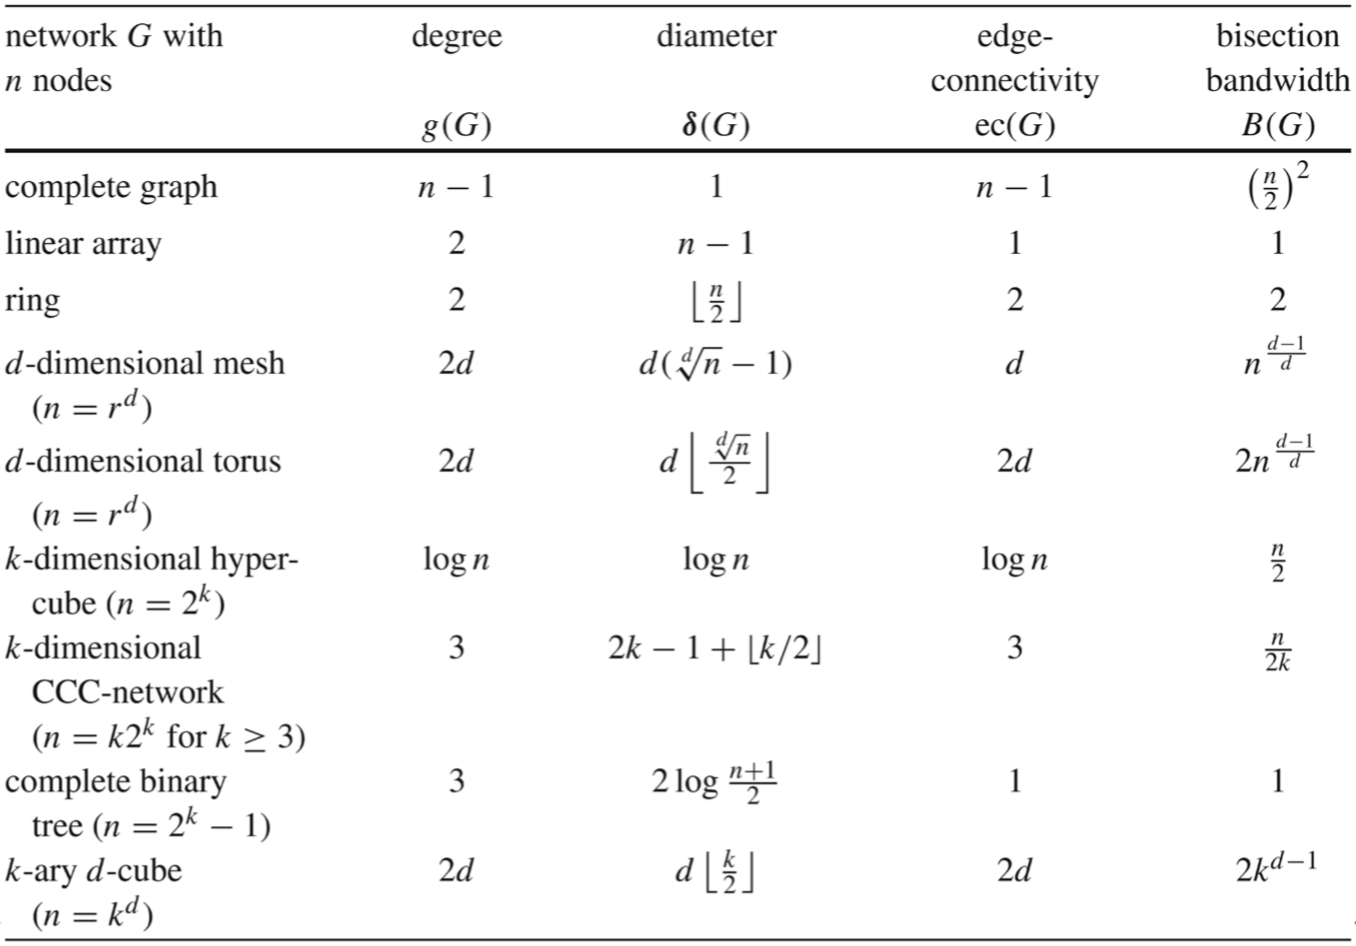
\includegraphics[scale=0.38]{./metrics}

\subsubsection{Indirect Interconnect}
\begin{itemize}
	\item Bus Network
	\item Crossbar Network - $n \times m$ switches
	\item Multistage Switching Network
		\begin{itemize}[label=$\circ$]
			\item Omega network 
				\begin{itemize}[label=$\ast$]
					\item $n \times n$ Omega network has $\log n$ stages
					\item $\frac{n}{2}$ switches per stage
					\item Switch position: ($\alpha$, $i$)
					\item $\alpha$: position of switch within a stage
					\item $i$: stage number
					\item Edge between ($\alpha$, $i$) and ($\beta$, $i+1$) where
					\item $\beta = \alpha$ by a cyclic left bit shift
					\item $\beta = \alpha$ by a cyclic left bit shift + inversion of LSBit
				\end{itemize}
			\item Butterfly network
				\begin{itemize}[label=$\ast$]
					\item Should be same number of switches and stages as Omega
					\item Node ($\alpha$, $i$) connects to:
					\item ($\alpha$, $i+1$), straight edge
					\item ($\alpha'$, $i$), $\alpha$ and $\alpha'$ differ in the $(i+1)$th bit from the left, i.e. cross edge
				\end{itemize}
			\item Baseline network
		\end{itemize}
\end{itemize}

\subsection{Routing}
\subsubsection{Classification}
\begin{itemize}
	\item Based on \textbf{path length}
		\begin{itemize}[label=$\ast$]
			\item \textbf{Minimal} or \textbf{Non-minimal} routing: whether \textbf{shortest path} is always chosen
		\end{itemize}
	\item Based on \textbf{adaptivity}
		\begin{itemize}[label=$\ast$]
			\item \textbf{Deterministic}: Always same path for same pair of (source, destination) node
			\item \textbf{Adaptive}: May take into account network status and adapt accordingly, e.g. avoid congested path, avoid dead nodes, etc.
		\end{itemize}
\end{itemize}

\subsubsection{XY Routing for 2D Mesh}
\begin{itemize}
	\item $(X_{src}, Y_{src}) \rightarrow (X_{dst}, Y_{dst})$
	\item Move in X direction until $X_{src} == X_{dst}$
	\item Move in Y direction until $Y_{src} == Y_{dst}$
\end{itemize}

\subsubsection{E-Cube Routing for Hypercube}
\begin{itemize}
	\item $(\alpha_{n-1}, \alpha_{n-2}, \dots, \alpha_{1}, \alpha_{0}) \rightarrow (\beta_{n-1}, \beta_{n-2}, \dots, \beta_{1}, \beta_{0})$
	\item Start from MSB to LSB (or LSB to MSB)
	\item Find first different bit
	\item Go to the neighboring node with the bit corrected
	\item \textbf{At most n hops}
\end{itemize}

\subsubsection{XOR-Tag Routing for Omega Network}
\begin{itemize}
	\item Let $T = $ Source Id $\oplus$ Destination Id
	\item At stage-$k$:
	\item Go straight if bit $k$ of T is 0
	\item Crossover if bit $k$ of T is 1
\end{itemize}

\rule{0.3\linewidth}{0.25pt}
\scriptsize
Copyright \copyright\ 2018 Edmund Mok

\end{multicols}
\end{document}
